\documentclass[journal]{IEEEtran}

\usepackage{graphicx}

\usepackage{listings}
\usepackage{xcolor}

% https://tex.stackexchange.com/questions/116534/lstlisting-line-wrapping
\lstset{
    frame=single,
    breaklines=true,
    postbreak=\mbox{\textcolor{red}{$\hookrightarrow$}\space},
}

\usepackage{csvsimple}
\usepackage{hyperref}

% https://tex.stackexchange.com/questions/534/is-there-any-way-to-do-a-correct-word-count-of-a-latex-document
\immediate\write18{texcount -inc -sum -1 assignment.tex > wordcount.tmp}
\newcommand\wordcount{
    \input{wordcount.tmp}
}

\newcommand{\codelisting}[2]{
    \texttt{#1}
    \lstinputlisting{#2}
}

\begin{document}

% Cover sheet
%TC: ignore
{\Large \textbf{Cover Sheet}}

Kieran Knowles

w20013000

Computer Science

Intelligent Systems KF5042

Submission date: \today

Word count: \wordcount

\title{A Comparative Study of the Impact of Emphasis of Sentiments in Training Data on the Performance of a Sentiment Analysis Model}
\author{Kieran Knowles}
\maketitle

%TC: endignore

\begin{abstract}
    //TODO: This

\end{abstract}

\section{Introduction}
This paper aims to study how the emphasis of sentiments in training data can impact the performance of a sentiment analysis
model. The hypothesis is that having more emphasised emotions in training data can improve the performance of the resulting
model, even when running on less emphasised speech.

While computer sentiment analysis has existed for decades \cite{stone_computer_1963}, existing research has primarily focused on
its use with text rather than speech. //TODO: Source

This review is incomplete however as it doesn't cover how the emphasis of sentiments in training data impacts the performance of a model.
Whilst researching this subject, no papers on the subject were found.
This could be because "audio sentiment analysis is still in a nascent stage
in the research community". \cite{maghilnan_sentiment_2017}

//TODO: This

\section{Literature Review}

//TODO: This

As the purpose of this study was to determine how the emphasis of speech affects
the performance of a model, only the audio from the training data was used as input,
for the model despite hybrid models being more accurate. \cite{bhaskar_hybrid_2015}

\subsection{Algorithm Selection}
A bidirectional Long Short-Term Memory (BLSTM) model was selected for this study as previous studies
have found that "the proposed LSTM-based technique leads to the best average recognition performance
that has been reported for this task so far." \cite{wollmer_lstm-modeling_2013}

\subsection{Training Data}
Video games have previously been used as training data for sentiment analysis models, such as in
Hämäläinen et al.'s paper, \cite{hamalainen_video_2022} which used Fallout New Vegas as training data.

This study uses the games Fallout New Vegas \cite{noauthor_buy_nodate} and
The Elder Scrolls IV: Oblivion \cite{noauthor_elder_nodate} as training data as
Oblivion uses the same system in which every line of dialogue is annotated with one of seven sentiments
(anger, disgust, fear, happy, neutral, sad, and surprised) and the game is voiced in three of the same five languages
(English, French, and German. The Spanish and Italian versions use the same voices as the English version).

For both of these games, the Microsoft Store versions were used as these include all available languages
in the same download. This simplified the process of downloading the data before extracting it.

Oblivion is known for sometimes having over-emphasised emotions in its dialogue.
This over-emphasis could be due to how the game's voice actors were given their lines
in alphabetical order. \cite[1:00]{noclip_-_video_game_documentaries_music_2018}

Fallout New Vegas was chosen as a second dataset as it uses a similar system, which
allows for similar code to be used to extract the data from both games.

\subsection{Limitations}
Human emotion is more complex than the per-line classifications used in this study and is instead
"a continuum" and that "common sense and psychological studies suggest that the full spectrum of
human emotion cannot be expressed by a few discrete classes" \cite{wollmer_abandoning_2008}

As the data used in this study only contains per-line classifications with seven possible emotions,
this is a limitation of the study that cannot be overcome with the data that is used.

\section{Methods}
\subsection{Considerations}
//TODO: This. Lack of actor variety, copyright (maybe in results and discussion)

Some lines of dialogue have actor notes which provided additional context to
the voice actors. These notes may lead actors to show a sentiment that does not
match the emotion annotated in the dialogue itself.

Additionally, the neutral emotion is the default emotion for any new line in the editor.
Because of this, some lines were never annotated with a sentiment despite the recorded
dialogue showing a specific emotion. See table \ref{table:bad_annotation}

\begin{table}[h]
    \begin{tabular}{| c | l |}
        \hline
        Text & Don't try to manipulate me. \\ \hline
        Annotation & Neutral \\ \hline
        File & oblivion.esm\textbackslash nord\textbackslash f\textbackslash generic\textunderscore admirehate\textunderscore 00062311\textunderscore 1.mp3 \\ \hline
        Actual emotion & Anger \\ \hline
    \end{tabular}
    \caption{An example of a lines annotation not matching the recording}
    \label{table:bad_annotation}
\end{table}

\subsection{Data Extraction}
Due to the instability of Fallout New Vegas' official tools as reported by Hämäläinen et al., \cite{hamalainen_video_2022},
which was assumed to be the same for Oblivion, the data was instead extracted using a custom script
written using the Mutagen library. \cite{noauthor_mutagen_2023}
This script outputs a CSV file containing the dialogue, the sentiment, and its extracted file path.

See tables \ref{table:category_counts_oblivion} and \ref{table:category_counts_new_vegas} for a breakdown of the number of samples in each category.

The data extraction script outputs a CSV file that can then be imported into MATLAB.

The "Pained" sentiment was removed from the New Vegas dataset as it does not exist in Oblivion and could therefore
interfere with the comparison between the two datasets.

//TODO: This
\begin{table}[h]
    \begin{center}
        \begin{tabular}{| c | c | c |}
            \hline
            Category & Sample Count & Proportion
            \csvreader[head to column names]{src/out/category_counts_oblivion.csv}{}%
            {\\ \hline \Name & \Count & \Proportion}%
            \\ \hline
        \end{tabular}
        \caption{The number of samples in each category for Oblivion}
        \label{table:category_counts_oblivion}
    \end{center}
\end{table}

\begin{table}[h]
    \begin{center}
        \begin{tabular}{| c | c | c |}
            \hline
            Category & Sample Count & Proportion
            \csvreader[head to column names]{src/out/category_counts_new_vegas.csv}{}%
            {\\ \hline \Name & \Count & \Proportion}%
            \\ \hline
        \end{tabular}
        \caption{The number of samples in each category for New Vegas}
        \label{table:category_counts_new_vegas}
    \end{center}
\end{table}

\subsection{Network Architecture}
The network consists of a single BiLSTM layer with 512 hidden units and outputs the last time step.
Dropout layers with a rate of 0.2 for the input and 0.5 for the output are used before and after
the BiLSTM layer to prevent overfitting. \cite{hinton_improving_2012}

This is then followed by a fully connected layer with one output for each
sentiment in the dataset (seven for Oblivion and eight for New Vegas).

The output of this layer is then passed through a softmax layer then a classification layer
to produce the final output.

See figure \ref{fig:network} for a visualisation of the network architecture.

The network was trained with a learning rate of 0.01 for 100 epochs. See //TODO: Results for the training and loss curves.

\begin{figure}
    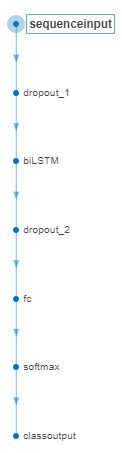
\includegraphics{network.png}
    \caption{The network architecture}
    \label{fig:network}
\end{figure}

\subsection{Training}
Due to limited memory, the neutral samples from both datasets were trimmed down to 20,000
samples for each dataset through random sampling. The remaining samples were then split into training and test sets
with a 95\%/5\% split. The small size of the test set was chosen due to the large size of the training set.

The neutral samples were selected for trimming as they made up a significant proportion of both
datasets, more so for New Vegas than Oblivion. See tables \ref{table:category_counts_oblivion}
and \ref{table:category_counts_new_vegas} for the exact proportions.

The low size for the test and validation sets was chosen due to the large size of the training set,
even after the neutral samples were trimmed down.

\section{Results and Discussion}
//TODO: This

\section{Conclusion and future work}
//TODO: This

%TC: ignore

\section*{Appendix}
\subsection*{Source Code}
% //TODO: This

\codelisting{load\textunderscore and \textunderscore transform.m}{src/load_and_transform.m}
\codelisting{load\textunderscore data.m}{src/load_data.m}
\codelisting{remove\textunderscore nans.m}{src/remove_nans.m}
\codelisting{run\textunderscore all.m}{src/run_all.m}
\codelisting{split\textunderscore data.m}{src/split_data.m}
\codelisting{train\textunderscore single.m}{src/train_single.m}
\codelisting{trim\textunderscore category.m}{src/trim_category.m}
\codelisting{write\textunderscore counts\textunderscore table.m}{src/write_counts_table.m}

\bibliographystyle{IEEEtran}
\bibliography{assignment}

%TC: endignore

\end{document}
